%% Copyright (C) 2021 Alessandro Clerici Lorenzini
%
% This work may be distributed and/or modified under the
% conditions of the LaTeX Project Public License, either version 1.3
% of this license or (at your option) any later version.
% The latest version of this license is in
%   http://www.latex-project.org/lppl.txt
% and version 1.3 or later is part of all distributions of LaTeX
% version 2005/12/01 or later.
%
% This work has the LPPL maintenance status `maintained'.
%
% The Current Maintainer of this work is Alessandro Clerici Lorenzini
%
% This work consists of the files listed in work.txt


% TODO: valutare le funzioni (ripartizione e massa) nel dominio negativo
\section{Modelli di distribuzione}
I modelli di distribuzione consistono in risultati notevoli corrispondenti a variabili aleatorie che rispettano determinate definizioni ricorrenti.

% TODO: bisognerebbe aggiungere anche il supporto, tuttavia non riesco a sistemare la geometria della pagina in un modo soddisfacente che non causi warning.
% TODO: per quelli non visti, è sufficiente fare le somme delle funzioni di massa. Per il problema di spazio già citato, per ora sono omesse
% TODO: controllare la mancanza di funzioni indicatrici
\begin{sidewaystable}
	\centering
	\begin{tabular}{llllll}
		\toprule
		\bfseries Modello           & \bfseries Parametri   & \bfseries F. di massa/densità                                    & \bfseries F. di ripartizione                                                                                          & \bfseries V. atteso & \bfseries Varianza    \\
		\midrule
		\bfseries Bernoulli         & $X\sim B(p)$          & $p^x(1-p)^{1-x}I_{\{0,1\}}(x)$                                   & $\begin{cases}0\quad & x<0\\1-p\quad & 0\leq x<1\\1\quad & x\leq 1\end{cases}$                                                                                           & $p$                 & $p(1-p)$              \\[5ex]
		\bfseries Binomiale         & $X\sim B(n,p)$        & $\displaystyle\binom{n}{i} p^i(1-p)^{n-i}$                       & $\begin{cases}\sum_{i=0}^{\floor{x}}\binom{n}{i} p^i (1-p)^{n-i}\quad & x\leq n \\1 & x>n \end{cases}$                                                                                           & $np$                & $np(1-p)$             \\[3ex]
		\bfseries Uniforme discreto & $X\sim U(n)$          & $\dfrac{1}{n} I_{\{1,\dots,n\}}(i)$                              & $\dfrac{\floor{x}}{n}\cdot I_{\{1,\dots,n\}}+I_{\{n,\dots,+\infty\}}$                                                 & $\dfrac{n+1}{2}$    & $\dfrac{n^2-1}{12}$   \\[2ex]
		\bfseries Geometrico        & $X\sim G(p)$          & $(1-p)^ip ~ I_\N (i)$                                            & $1 - (1-p)^{\floor{x}+1}  $                                                                                           & $ \dfrac{1-p}{p}$   & $\dfrac{1-p}{p^2}$    \\[1ex]
		\bfseries Poisson           & $X\sim P(\lambda)$    & $e^{-\lambda}\frac{\lambda^i}{i!} ~ I_\N(i)$                     & [non visto]                                                                                                           & $\lambda$           & $\lambda$             \\[2ex]
		\bfseries Ipergeometrico    & $X\sim ?(N,M,n)$      & $\dfrac{\binom{N}{i}\binom{M}{n-i}}{\binom{N+M}{n}}$             & [non visto]                                                                                                           & $np$                & $\dfrac{NM}{(N+M)^2}$ \\[2ex]
		\bfseries Uniforme continuo & $X\sim U([a,b])$      & $\dfrac{1}{b-a} I[a,b](x)$                                       & $ \dfrac{x-a}{b-a}\cdot I_{[a,b]}(x)+I_{(b,+\infty)}(x)$                                                              & $\dfrac{b+a}{2}$    & $\dfrac{(b-a)^2}{12}$ \\[3ex]
		\bfseries Esponenziale      & $X\sim E(\lambda)$    & $\lambda e^{-\lambda x} I_{\R^+}(x)$                             & $1-e^{-\lambda x}$                                                                                                    & $\frac{1}{\lambda}$ & $\frac{1}{\lambda^2}$ \\[1ex]
		\bfseries Gaussiano         & $X\sim N(\mu,\sigma)$ & $\dfrac{1}{\sqrt{2\pi}~\sigma}e^{-\dfrac{(x-\mu)^2}{2\sigma^2}}$ & $\displaystyle\int_{-\infty}^x \dfrac{1}{\sqrt{2\pi}~\sigma} e^{-\frac{1}{2}\left(\dfrac{y-\mu}{\sigma}\right)^2} dy$ & $\mu$               & $\sigma^2$            \\
		\bottomrule
	\end{tabular}
	\caption{Tabella riassuntiva dei modelli di distribuzione.}
\end{sidewaystable}

\begin{sidewaysfigure}
\begin{center}
	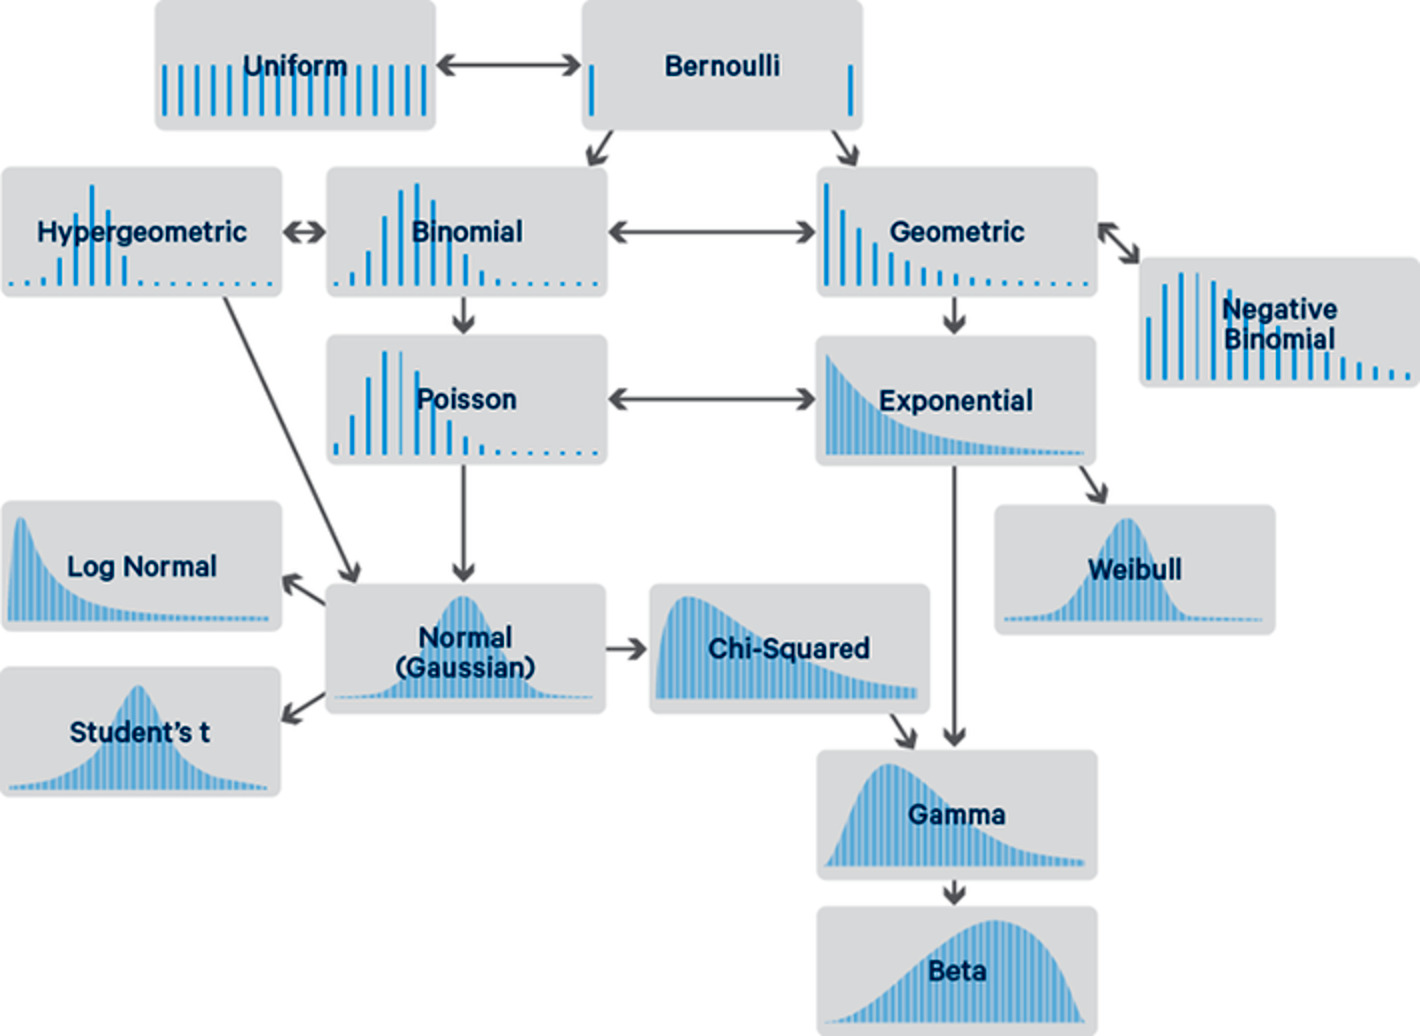
\includegraphics[scale=0.4]{models}
	\end{center}
\end{sidewaysfigure}

\subsection{Modello bernoulliano}
Il modello bernoulliano impone alle sue variabili aleatorie di avere specificazione binaria, cioè $D_X=\{0,1\}$ per qualunque variabile $X$.

Una variabile aleatoria bernoulliana di probabilità di successo ($X=1$) $p$ si indica con
\begin{equation*}
	X\sim B(p)
\end{equation*}
mentre il fallimento è rappresentato da $(X = 0)$\\
\footnotesize{Brutalmente: quando gli esiti sono binari: il fallimento è rappresentato da 0 ed il successo da 1, stiamo parlando di un modello di bernoulli)
\normalsize

\subsubsection{Funzione di massa di probabilità}
La funzione di massa di probabilità di una variabile aleatoria bernoulliana è
\begin{equation*}
	p_X(x)=P(X=x)=p^x(1-p)^{1-x}I_{\{0,1\}}(x)=\begin{cases}
		1-p \qquad & x=0               \\
		p \qquad   & x=1               \\
		0 \qquad   & \text{altrimenti}
	\end{cases}
\end{equation*}


\subsubsection{Valore atteso}
In analogia con la proprietà \ref{prop:indvalatt}, il valore atteso di una variabile aleatoria bernoulliana è $p$:
\begin{equation*}
	\ev{X} = p
\end{equation*}
E ovviamente
\begin{equation*}
	\ev{X^2}=\ev{X}
\end{equation*}


\subsubsection{Varianza}
In analogia con la proprietà \ref{prop:indvar}, la varianza di una variabile aleatoria bernoulliana è $p(1-p)$:
\begin{equation*}
	\var(X) = p(1-p)
\end{equation*}


\subsubsection{Funzione di ripartizione}
La funzione di ripartizione per variabili bernoulliane è ovviamente uguale a $0$ per $x<0$, $1-p$ per $0\leq x<1$ e $1$ per $x\geq 1$.



\subsection{Modello binomiale}
Il modello binomiale consiste in $n$ ripetizioni di un esperimento bernoulliano di probabilità $p$. Una variabile aleatoria binomiale corrisponde al numero di successi tra gli $n$ esperimenti.
\begin{equation*}
	X \sim B(n, p)\qquad D_X=\{0,1,\dots,n\}
\end{equation*}


\subsubsection{Funzione di massa di probabilità}
Per definizione:
\begin{equation*}
	p_X(i) = P(X=i)
\end{equation*}
Tale probabilità è l'intersezione degli eventi indipendenti che consistono nel successo dal primo all'$i$-esimo e insuccesso dall'$i+1$-esimo all'$n$-esimo. In quanto probabilità di eventi indipendenti, essa può essere espressa come il prodotto delle singole probabilità. Ognuna delle probabilità di successo, per come è costruito il modello binomiale, è $p$, mentre ognuna delle probabilità di insuccesso è $1-p$. Ogni combinazione in cui $i$ esperimenti hanno successo e $n-i$ falliscono è valida, perciò:
\begin{equation}
	P(X=i) = \binom{n}{i} p^i(1-p)^{n-i}
\end{equation}

Concorde con la \eqref{eq:sommamassa}, la somma delle immagini della funzione di massa di probabilità è 1:
\begin{equation*}
	\sum_{i=1}^n p_X(i) = \sum_{i=1}^n \binom{n}{i} p^i(1-p)^{n-i} = (p+1-p)^n = 1
\end{equation*}


\subsubsection{Valore atteso}
Essendo ogni variabile aleatoria binomiale la somma di variabili aleatorie bernoulliane:
\begin{equation}
	\ev{X} = \ev{\sum_{i=0}^n X_i} = \sum_{i=0}^n \ev{X_i} = \sum_{i=0}^n p = np
\end{equation}


\subsubsection{Varianza}
Essendo le componenti bernoulliane indipendenti:
\begin{equation}
	\var(X)=\sum_{i=1}^n \var(X_i) = \sum_{i=1}^n p(1-p) = np(1-p)
\end{equation}


\subsubsection{Funzione di ripartizione}
Per calcolare con un'unica formula la funzione di ripartizione si aggiungono due funzioni indicatrici, che agiscono se $x>n$:
\begin{align}
	F_X(x) & = P(X\leq x)                                                                           \nonumber            \\
	       & = I_{(n,+\infty)}(x) + I_{[0,n]}(x) \sum_{i=0}^{\floor{x}}\binom{n}{i} p^i (1-p)^{n-i} \label{eq:ripabinom} \\
	       & = \begin{cases}
		\sum_{i=0}^{\floor{x}}\binom{n}{i} p^i (1-p)^{n-i}\quad & x\leq n \\
		1                                                       & x>n     \\
	\end{cases} \nonumber
\end{align}

\subsubsection{Relazioni tra variabili binomiali}
Siano $X_1$ e $X_2$ due variabili aleatorie definite su modelli binomiali che differiscono solo per il numero di esperimenti:
\begin{align*}
	 & X_1\sim B(n, p)\quad & X_1=\sum_{i=1}^n X_{1,i}\qquad & X_{1,i}\sim B(p)~\forall i\in\{1,\dots,n\} \\
	 & X_2\sim B(m, p)\quad & X_1=\sum_{j=1}^m X_{2,j}\qquad & X_{2,j}\sim B(p)~\forall j\in\{1,\dots,m\}
\end{align*}

\noindent
Se $X_1$ e $X_2$ sono indipendenti, allora:
\begin{equation*}
	X_1+X_2 = \sum_{i=1}^n X_{1,i} + \sum_{j=1}^m X_{2,j} = \sum_{i=1}^{n+m} Y_i = Y
\end{equation*}
dove $Y\sim B(n+m, p)$.



\subsection{Modello uniforme discreto} \label{subsec:unifdisc}
Nel modello uniforme discreto le variabili aleatorie consistono nell'esito di un esperimento da $n$ esiti possibili equiprobabili:
\begin{equation*}
	X\sim U(n)
\end{equation*}


\subsubsection{Funzione di massa di probabilità}
Essendo gli $n$ esiti equiprobabili, la funzione di massa di probabilità assume il valore $\frac{1}{n}$ per tutti i valori dell'input compresi tra gli esiti (numerati qui da $1$ a $n$):
\begin{equation*}
	p_X(i) = P(X=i) = \frac{1}{n} I_{\{1,\dots,n\}}(i)
\end{equation*}


\subsubsection{Funzione di ripartizione}
\begin{equation*}
	\forall x\leq n\qquad F_X(x) = P(X\leq x) = \sum_{i=1}^{\floor{x}} P(X=i) = \sum{i=1}^{\floor{x}} \frac{1}{n} = \frac{\floor{x}}{n}
\end{equation*}
Come per la \eqref{eq:ripabinom}, si aggiungono funzioni indicatrici per regolare il valore oltre $n$:
\begin{equation}
	F_X(x)=\frac{\floor{x}}{n} I_{[1,n]}(x)+I_{(n,+\infty)}(x)
\end{equation}


\subsubsection{Valore atteso}
Banalmente, usando la definizione:
\begin{equation} \label{eq:disunvalat}
	\ev{X} = \sum_{i=1}^n i P(X=i) = \frac{1}{n} \sum_{i=1}^n i = \frac{1}{n}\frac{n(n+1)}{2} = \frac{n+1}{2}
\end{equation}


\begin{equation*}
	\ev{X^2} = \sum_{i=1}^{n}\frac{i^2}{n} = \frac{1}{n}\sum_{i=1}^{n}i^2=\frac{(n+1)(2n+1)}{6}
\end{equation*}


\subsubsection{Varianza}
Usando la definizione equivalente di varianza e quanto appena calcolato:
\begin{align*}
	\var(X) & = \ev{X^2} - \ev{X}^2 =                                       \bc{proprietà \ref{prop:varalt}}           \\
	        & = \sum_{i=1}^n i^2 P(X=i) - \left(\frac{n+1}{2}\right)^2      \bc{valore atteso e \eqref{eq:disunvalat}} \\
	        & = \frac{1}{n} \sum_{i=1}^n i^2 - \left(\frac{n+1}{2}\right)^2 \bc{ipotesi di equiprobabilità}            \\
	        & = \frac{(n+1)(2n+1)}{6}-\left(\frac{n+1}{2}\right)^2          \bc{somma notevole}                        \\
	        & = (n+1)\left(\frac{2n+1}{6}+\frac{n+1}{4}\right)              \bc{raccogliendo $n+1$}                    \\
	        & = (n+1)\left(\frac{n-1}{12}\right)                                                                       \\
	        & = \frac{n^2-1}{12}
\end{align*}



\subsection{Modello geometrico}
Una variabile aleatoria geometrica corrisponde al numero di insuccessi prima del primo successo in una sequenza di esperimenti bernoulliani con lo stesso parametro $p$ e tra loro indipendenti.

Per $p=0$ non si ottiene mai un successo, pertanto la variabile geometrica non è definita. Per $p=1$ la variabile assume necessariamente il valore $0$.

Il supporto di una variabile geometrica è l'insieme dei naturali.

\begin{equation*}
	X\sim G(p)\qquad D_X=\N
\end{equation*}


\subsubsection{Funzione di massa di probabilità}
La funzione di massa di probabilità in $i$ è uguale alla probabilità di insuccesso per ognuna delle $i$ ripetizioni indipendenti per la probabilità di successo della $i+1$-esima.

Come sempre si aggiunge una funzione indicatrice per aggiustare il dominio di $F_X$:
\begin{equation} \label{eq:geommasprob}
	F_X(i) = P(X=i) = (1-p)^ip ~ I_{N\cup\{0\}} (i)
\end{equation}

La somma delle immagini della funzione di massa di probabilità converge, come dovrebbe, a $1$:
\begin{align*}
	\sum_{i=0}^{+\infty} P(X=i) & = \sum_{i=0}^{+\infty} p(1-p)^i \\
	                            & = p\sum_{i=0}^{+\infty} (1-p)^i \\
	                            & = p\frac{1}{1-(1-p)}            \\
	                            & = 1
\end{align*}


\subsubsection{Valore atteso}
Tramite la definizione:
\begin{align*}
	\ev{X} & = \sum_{i=0}^{+\infty} i P(X=i)                    \bc{definizione \ref{def:valatt}}         \\
	       & = \sum_{i=0}^{+\infty} ip(1-p)^i                   \bc{\eqref{eq:geommasprob}}               \\
	       & = p(1-p)\sum_{i=0}^{+\infty} i(1-p)^{i-1}                                                    \\
	       & = -p(1-p) \frac{d}{dx} \sum_{i=0}^{+\infty} (1-p)^i \bc{derivata di $(1-p)^i$ e della somma} \\
	       & = -p(1-p) \frac{d}{dx} \frac{1}{p}                  \bc{serie geometrica di ragione $1-p$}   \\
	       & = \frac{p(1-p)}{p^2} = \frac{1-p}{p}                 \bc{derivando}
\end{align*}


\subsubsection{Varianza}
Volendo usare la forma equivalente \eqref{eq:varalt} di cui alla proprietà \ref{prop:varalt}, si calcola innanzitutto il valore atteso del quadrato della variabile:
\begin{align*}
	\ev{X^2} & = \sum_{i=0}^{+\infty} i^2 p(1-p)^i                                                                                                          \\
	         & = p(1-p) \sum_{i=0}^{+\infty} i^2 (1-p)^{i-1}                                                                                                \\
	         & = -p(1-p) \sum_{i=0}^{+\infty} i \frac{d}{dp}(1-p)^i \bc{derivata di $(1-p)^i$}                                                              \\
	         & = -p(1-p) \frac{d}{dp}\sum_{i=0}^{+\infty} i (1-p)^i \bc{\parbox{42.5mm}{prodotto di una derivata per una costante e derivata di una somma}} \\
	         & = -p(1-p) \frac{d}{dp}(1-p)\sum_{i=0}^{+\infty} i (1-p)^{i-1}                                                                                \\
	         & = p(1-p) \frac{d}{dp}(1-p) \frac{d}{dp} \sum_{i=0}^{+\infty} (1-p)^i                                                                         \\
	         & = -p(1-p) \frac{d}{dp} \frac{1-p}{p^2}                                                                                                       \\
	         & = -p(1-p) \frac{-p^2-2p(1-p)}{p^4}                                                                                                           \\
	         & = (1-p) \frac{p+2(1-p)}{p^2}                                                                                                                 \\
	         & = \frac{(1-p)(2-p)}{p^2}
\end{align*}
Da cui:
\begin{align*}
	\var(X) & = \ev{X^2}-\ev{X}^2                                     \\
	        & = \frac{(1-p)(2-p)}{p^2} - \left(\frac{1-p}{p}\right)^2 \\
	        & = \frac{(1-p)((2-p)-(1-p))}{p^2}                        \\
	        & = \frac{1-p}{p^2}
\end{align*}


\subsubsection{Funzione di ripartizione}
\begin{align*}
	F_X(n) & = P(X\leq n) = 1-P(X>n) =                                                                                                 \\
	       & = 1 - \sum_{i=n+1}^{+\infty} P(X=i)                                                                                       \\
	       & = 1 - \sum_{i=n+1}^{+\infty} p(1-p)^i                                                                                     \\
	       & = 1 - p(1-p)^{n+1} \sum_{i=n+1}^{+\infty} (1-p)^{i-(n+1)} \justif{~}{moltiplicando per $\frac{(1-p)^{n+1}}{(1-p)^{n+1}}$} \\
	       & = 1 - p(1-p)^{n+1} \sum_{i=0}^{+\infty} (1-p)^i \justif{~}{sostituzione: $i=i-(n+1)$}                                     \\
	       & = 1 - p(1-p)^{n+1} \frac{1}{1-(1-p)}                                                                                      \\
	       & = 1 - (1-p)^{n+1}                                                                                                         \\
\end{align*}
Questo risultato è in realtà banale se si applica il concetto semantico alla variabile geometrica.

\begin{equation*}
	F_X(x) = P(X\leq x) = 1-P(X>x) = 1-(1-p)^{\floor{x}+1}
\end{equation*}


\subsubsection{Assenza di memoria} \label{geom-assmem}
Come si può intuire, la probabilità di costante insuccesso all'$i+j$-esimo esperimento non è condizionata dalla probabilità di costante insuccesso all'$i$-esimo. Questo risultato prende il nome di assenza di memoria.
\begin{align*}
	P(X\geq i+j \mid X\geq i) & = \frac{P(X\geq i+j \cap X\geq i)}{P(X\geq i)} \\
	                          & = \frac{P(X\geq i+j)}{P(X\geq i)}              \\
	                          & = \frac{(1-p)^{i+j}}{(1-p)^i}                  \\
	                          & = (1-p)^j                                      \\
	                          & = P(X\geq j)
\end{align*}



\subsection{Modello di Poisson}
\begin{equation*}
	X\sim P(\lambda) \qquad D_X = \N \qquad \lambda>0
\end{equation*}

\subsubsection{Funzione di massa di probabilità}
\begin{equation*}
	P_X(i) = P(X=i) = e^{-\lambda}\frac{\lambda^i}{i!} ~ I_\N(i)
\end{equation*}

Ancora una volta la somma delle immagini della funzione di massa di probabilità converge a $1$:
\begin{equation} \label{eq:poisummas}
	\sum_{i=0}^{+\infty} e^{-\lambda}\frac{\lambda^i}{i!} = e^{-\lambda}\sum_{i=0}^{+\infty} \frac{\lambda^i}{i!} = e^{-\lambda}e^\lambda = 1
\end{equation}


\subsubsection{Valore atteso}
Tramite la definizione:
\begin{align}
	\ev{X} & = \sum_{i=0}^{+\infty} i P(X=i) = \sum_{i=1}^{+\infty} i P(X=i) \bc{definizione \ref{def:valatt}} \nonumber \\
	       & = \sum_{i=1}^{+\infty} i e^{-\lambda}\frac{\lambda^i}{i!} \label{eq:poinotevolelambda}                      \\
	       & = \lambda e^{-\lambda} \sum_{i=1}^{+\infty} \frac{\lambda^{i-1}}{(i-1)!} \nonumber                          \\
	       & = \lambda e^{-\lambda} \sum_{i=0}^{+\infty}\frac{\lambda^i}{i!} \bc{sostituzione: $i=i-1$} \nonumber        \\
	       & = \lambda e^{-\lambda} e^\lambda \nonumber                                                                  \\
	       & = \lambda
\end{align}


\subsubsection{Varianza}
Volendo usare la forma equivalente \eqref{eq:varalt}, si calcola innanzitutto il valore atteso di $X^2$:
\begin{align*}
	\ev{X^2} & = \sum_{i=1}^{+\infty} i^2 e^{-\lambda}\frac{\lambda^i}{i!}                                                                                                                              \\
	         & = \sum_{i=1}^{+\infty} i e^{-\lambda} \frac{\lambda^i}{(i-1)!}                                                                                                                           \\
	         & = \lambda\sum_{i=1}^{+\infty} i e^{-\lambda}\frac{\lambda^{i-1}}{(i-1)!}                                                                                                                 \\
	         & = \lambda\sum_{i=1}^{+\infty} (i-1+1) e^{-\lambda}\frac{\lambda^{i-1}}{(i-1)!}                                                                                                           \\
	         & = \lambda\sum_{i=1}^{+\infty}\left((i-1)e^{-\lambda}\frac{\lambda^{i-1}}{(i-1)!}+e^{-\lambda}\frac{\lambda^{i-1}}{(i-1)!}\right)                                                         \\
	         & = \lambda\sum_{i=1}^{+\infty} (i-1)e^{-\lambda}\frac{\lambda^{i-1}}{(i-1)!} + \lambda\sum_{i=1}^{+\infty} + e^{-\lambda}\frac{\lambda^{i-1}}{(i-1)!}                                     \\
	         & = \lambda\underbrace{\sum_{i=0}^{+\infty} ie^{-\lambda}\frac{\lambda^i}{i!}}_{\lambda} + \lambda \underbrace{\sum_{i=0}^{+\infty} e^{-\lambda}\frac{\lambda^i}{i!}}_{1} \bc{con $i=i-1$} \\
	         & = \lambda^2 + \lambda \bc{\eqref{eq:poinotevolelambda} e \eqref{eq:poisummas}}
\end{align*}
Ergo
\begin{align}
	\var(X) & = \ev{X^2} - \ev{X}^2         \nonumber \\
	        & = \lambda^2+\lambda-\lambda^2 \nonumber \\
	        & = \lambda
\end{align}

\subsubsection{Approssimazione del modello binomiale} \label{subsub:binompois}
Il modello di Poisson è strettamente legato al modello binomiale. Infatti, se il prodotto dei parametri di una binomiale è costante, per $n$ grandi essa è ben approssimata da una variabile di Poisson che ha come parametro tale prodotto:
\begin{equation*}
	X\sim B(n, p)\qquad\text{con }np=\lambda
\end{equation*}
Per $n\to+\infty$:
\begin{align*}
	P(X=i) & = \binom{n}{i} p^i (1-p)^{n-i}                                                                                                                                                                                                                                                \\
	       & = \binom{n}{i}\left(\frac{\lambda}{n}\right)^i\left(1-\frac{\lambda}{n}\right)^{n-i}                                                                                                                                                                                          \\
	       & = \frac{n(n-1) \dots (n-i+1)}{i!} \cdot \frac{\lambda^i}{n^i} \left( 1 - \frac{\lambda}{n} \right)^{n-i}                                                                                                                                                                      \\
	       & = \frac{n(n-1) \dots (n-i+1)}{n^i} \cdot \frac{\lambda^i}{i!} \left( 1 - \frac{\lambda}{n} \right)^{n-i}                                                                                                                                                                      \\
	       & = \underbrace{\frac{n}{n}}_{\to 1} \cdot \underbrace{\frac{n-1}{n}}_{\to 1} \dots \underbrace{\frac{n-i+1}{n}}_{\to 1} \cdot \frac{\lambda^i}{i!} \cdot \underbrace{\frac{\left( 1 - \frac{\lambda}{n} \right)^n}{\left( 1 - \frac{\lambda}{n} \right)^i}}_{\to e^{-\lambda}} \\
	       & \to \frac{\lambda^i}{i!} e^{-\lambda}
\end{align*}

\subsection{Riproducibilità}
\begin{center}
$x_1 \sim P (\lambda_1), x_2 \sim P(\lambda_2) \quad \rightarrow \quad x_1 + x_2 \sim P(\lambda_1 + \lambda_2)$
\end{center}


\subsection{Modello ipergeometrico}
Il modello ipergeometrico descrive il classico problema dell'urna. Dati $N$ oggetti funzionanti e $M$ oggetti difettosi, sia $n$ il numero di estrazioni senza reimmissione. La variabile aleatoria ipergeometrica X è il numero di oggetti funzionanti nelle $n$ estrazioni.
\begin{equation*}
	X\sim ?(?)
\end{equation*}
Il modello è valido solo se $P(X=0)=0$.

%todo: what is this


\subsubsection{Funzione di massa di probabilità}
Il numero di casi possibili sono le combinazioni di $n$ estrazioni senza reimmissione da un gruppo di $N+M$. Il numero di casi favorevoli si può calcolare applicando il principio fondamentale del calcolo combinatorio.
\begin{equation*}
	P(X=i) = \frac{\binom{N}{i}\binom{M}{n-i}}{\binom{N+M}{n}}
\end{equation*}


\subsubsection{Valore atteso}
Al fine di calcolare il valore atteso si sfrutta un approccio decomposizionale: si introducono $n$ variabili aleatorie $X_i$, ognuna legata a un'estrazione, tali che
\begin{equation*}
	X_i = \begin{cases}
		1 & \text{l'$i$-esimo oggetto estratto funziona} \\
		0 & \text{altrimenti}
	\end{cases}
\end{equation*}

Per tali variabili vale
\begin{equation*}
	P(X_i=1) = \frac{N}{N+M} =: p = \ev{X_i}
\end{equation*}

Da cui
\begin{align*}
	\ev{X} & = \ev{\sum_{i=1}^n X_i} \\
	       & = \sum_{i=1}^n \ev{X_i} \\
	       & = np
\end{align*}


\subsubsection{Varianza}
Applicando la proprietà \ref{prop:varalt} si calcola la varianza delle singole $X_i$:
\begin{align*}
	\var(X_i) & = \ev{X_i^2}-\ev{X_i}^2                                   \\
	          & = \ev{X_i}(1-\ev{X_i})          \bc{idempotenza di $X_i$} \\
	          & = \frac{N}{N+M} + \frac{M}{N+M}                           \\
	          & = \frac{NM}{(N+M)^2}
\end{align*}

Essendo le variabili $X_i$ non indipendenti, la varianza della loro somma non è uguale alla somma delle varianze. Si può comunque applicare la proprietà \ref{prop:varsumcov} e passare per le covarianze:
\begin{align*}
	\cov(X_i,X_j) & = \ev{X_i X_j} - \ev{X_i}\ev{X_j}                                \\
	              & = \ev{X_i=1\cap X_j=1} - \left(\frac{N}{N+M}\right)^2            \\
	              & = P(X_j=1 \mid X_i=1)P(X_i=1) - \left(\frac{N}{N+M}\right)^2     \\
	              & = \frac{N-1}{N+M-1} \frac{N}{N+M} - \left(\frac{N}{N+M}\right)^2 \\
	              & = \frac{N}{N+M} \left(\frac{N-1}{N+M-1} - \frac{N}{N+M}\right)   \\
	              & = \frac{-NM}{(N+M-1)(N+M)^2}
\end{align*}
Ergo
\begin{align*}
	\var(X) & = \sum_{i=1}^n \var(X_i) + \sum_{i\neq j}^n \cov(X_i,X_j)     \\
	        & = n\frac{NM}{(N+M)^2} - n(n-1)\cdot\frac{-NM}{(N+M-1)(N+M)^2} \\
	        & = n\frac{NM}{(N+M)^2}\left(1-(n-1)\frac{1}{N+M-1}\right)      \\
	        & = np(1-p)\left(1-\frac{n-1}{N+M-1}\right)
\end{align*}
Per $N+M\to+\infty$ il modello si semplifica in un modello binomiale:
\begin{equation*}
	\to np(1-p)
\end{equation*}


\subsection{Modello uniforme continuo}
Il modello uniforme continuo estende al continuo i concetti visti alla sezione \ref{subsec:unifdisc} per il modello uniforme discreto e viene determinato da un intervallo equivalentemente aperto o chiuso:
\begin{equation*}
	X \sim U([a,b]) \quad a < b \quad D_x = [a,b]
\end{equation*}


\subsubsection{Funzione di densità di probabilità}
\begin{equation*}
	f(X)(x) = \frac{1}{b-a} I[a,b](x)
\end{equation*}
essendo la densità costante, per $I\subseteq[a,b]$:
\begin{equation*}
	P(X\in I) = \frac{|I|}{b-a}
\end{equation*}
dove $|I|$ è la somma delle ampiezze $p-q$ degli intervalli disgiunti $[p,q]$ da cui $I$ è composto.

Come da definizione, integrando nell'intero $\R$ la funzione di densità di probabilità si ottiene $1$:
\begin{equation*}
	\int_{-\infty}^{+\infty}f_X(x) = \int_a^b\frac{1}{b-a}dx = \frac{1}{b-a} \eval{x}{a}{b} = 1
\end{equation*}


\subsubsection{Funzione di ripartizione}
Per definizione la funzione di ripartizione è la funzione integrale della funzione di densità:
\begin{align*}
	F_X(x) & = P(X\leq x)                   \\
	       & = \int_{-\infty}^x f_X(u)du    \\
	       & = \int_a^x \frac{1}{b-a}du     \\
	       & = \frac{1}{b-a} \eval{u}{a}{x} \\
	       & = \frac{x-a}{b-a}
\end{align*}
\footnotesize{}
$f_X(u)du$ perché la variabile non può essere uguale\\
\normalsize{}

Come sempre funzioni indicatrici aggiustano il risultato per punti non appartenenti all'intervallo:
\begin{equation*}
	F_X(x) = \frac{x-a}{b-a} I_{[a,b]}(x) + I_{(b,+\infty)}(x)
\end{equation*}


\subsubsection{Valore atteso}
Applicando la definizione:
\begin{align*}
	\ev{X} & = \int_a^b x f_X(x)dx                      \\
	       & = \frac{1}{b-a} \int_a^b x ~ dx            \\
	       & = \frac{1}{b-a} \eval{\frac{x^2}{2}}{a}{x} \\
	       & = \frac{1}{b-a} \cdot \frac{b^2-a^2}{2}    \\
	       & = \frac{b+a}{2}
\end{align*}
Che deriva dalla somma tra la area del rettangolo e l'area del triangolo nel grafico, che corrisponde anche al punto medio.


\subsubsection{Varianza}
Come di consueto si intende applicare la proprietà \ref{prop:varalt}, pertanto si calcola innanzitutto il valore atteso di $X^2$:
\begin{align*}
	\ev{X^2} & = \int_a^b x^2 f_X(x)dx                    \\
	         & = \frac{1}{b-a}\int_a^b x^2 ~ dx           \\
	         & = \frac{1}{b-a} \eval{\frac{x^3}{3}}{a}{b} \\
	         & = \frac{b^3-a^3}{3(b-a)}                   \\
	         & = \frac{a^2+ab+b^2}{3}
\end{align*}

E infine:
\begin{align*}
	\var(X) & = \ev{X^2} - \ev{X}^2                      \\
	        & = \frac{a^2+ab+b^2}{3} - \frac{(a+b)^2}{4} \\
	        & = \frac{(b-a)^2}{12}
\end{align*}


\subsection{Modello esponenziale}
Nel modello esponenziale la funzione di densità è esponenziale.
\begin{equation*}
	X\sim E(\lambda) \qquad \lambda\in\R^+ \quad D_X=\R^+
\end{equation*}


\subsubsection{Funzione di densità di probabilità}
\begin{equation*}
	f_X(x) = \lambda e^{-\lambda x} I_{\R^+}(x)
\end{equation*}

Il modello esponenziale si usa per modellare il tempo che intercorre tra due eventi.

La funzione di densità rispetta la definizione, infatti:
\begin{align*}
	\int_0^{+\infty} f_X(x)dx & = \int_0^{+\infty} \lambda e^{-\lambda x} dx       \\
	                          & = \int_0^{+\infty} e^{-y}dy \bc{con $y=\lambda x$} \\
	                          & = \eval{-e^{-y}}{0}{+\infty}                       \\
	                          & = 0 + e^{-0}                                       \\
	                          & = 1
\end{align*}


\subsubsection{Funzione di ripartizione}
Applicando la definizione di funzione di ripartizione continua:
\begin{align*}
	F_X(x) & = \int_0^x f_X(y)dy                                  \\
	       & = \int_0^x \lambda e^{\lambda y}dy                   \\
	       & = \int_0^{\lambda x} e^{-z}dz \bc{con $z=\lambda y$} \\
	       & = \eval{-e^{-z}}{0}{\lambda x}                       \\
	       & = -e^{-\lambda x} + e^0                              \\
	       & = 1-e^{-\lambda x}
\end{align*}
Aggiungendo una funzione indicatrice:
\begin{equation}
	F_X(x) = (1 - e^{-\lambda x})I_{\R^+}(x)
\end{equation}


\subsubsection{Valore atteso}
Applicando la definizione:
\begin{align*}
	\ev{X} & = \int_0^{+\infty} x f_X(x) dx                                                             \\
	       & = \int_0^{+\infty} x\lambda e^{-\lambda x}dx                                               \\
	       & = \eval{-x e^{-\lambda x}}{0}{+\infty} + \int_0^{+\infty} e^{-\lambda x} dx \bc{per parti} \\
	       & = \int_0^{+\infty} e^{-\lambda x} dx                                                       \\
	       & = \frac{1}{\lambda} \underbrace{\int_0^{+\infty} \lambda e^{-\lambda x}}_{1}               \\
	       & = \frac{1}{\lambda} \bc{proprietà di $f_X$}
\end{align*}


\subsubsection{Varianza}
Volendo usare la forma equivalente \eqref{eq:varalt}, si calcola innanzitutto il valore atteso di $X^2$:
\begin{align*}
	\ev{X^2} & = \int_0^{+\infty} x^2\lambda e^{-\lambda x} dx                                 \\
	         & = \eval{-x^2 e^{-\lambda x}}{0}{+\infty} + \int_0^{+\infty} 2xe^{-\lambda x} dx \\
	         & = 2\int_0^{+\infty} xe^{-\lambda x}dx                                           \\
	         & = \frac{2}{\lambda} \int_0^{+\infty} \lambda xe^{-\lambda x}dx                  \\
	         & = \frac{2}{\lambda} \ev{X} = \frac{2}{\lambda^2}
\end{align*}
Da cui:
\begin{align*}
	\var(X) & = \ev{X^2} - \ev{X}^2                                           \\
	        & = \frac{2}{\lambda^2}-\frac{1}{\lambda^2} = \frac{1}{\lambda^2}
\end{align*}


\subsubsection{Assenza di memoria}
Le variabili di modello esponenziale godono della proprietà di assenza di memoria (già vista per il modello geometrico al paragrafo \ref{geom-assmem}):
\begin{equation*}
	P(X>x) = 1 - F_X(x) = e^{-\lambda x}
\end{equation*}
Quindi:
\begin{align*}
	P(X>s+t) & = e^{-\lambda (s+t)}           \\
	         & = e^{-\lambda s}e^{-\lambda t} \\
	         & = P(X>s)P(X>t)
\end{align*}
Da cui
\begin{align*}
	P(X>s) & = \frac{P(X>s+t)}{P(X>t)}         \\
	       & = \frac{P(X>s+t\cap X>t)}{P(X>t)} \\
	       & = P(X>s+t\mid X>t)
\end{align*}
Le due espressioni coincidono logicamente. Possiamo estendere questa notazione:
\begin{align*}
P(x < x ) & = 1 - P(X \leq x ) = \\
		 & =1 - F_x = e ^{-\lambda x}
\end{align*}


\subsubsection{Corollario}
Consideriamo un modello esponenziale
\begin{center}
$X \sim E(\lambda) \quad Y := \alpha X \quad \alpha > 0$
\end{center}
\begin{align*}
F_y(x) &= P(Y \leq x) = P(\alpha X \leq x) = P(x \leq \frac{x}{\alpha})\\
	  & F_x(\frac{x}{\alpha}) = 1 - e^{-\lambda \frac{x}{\alpha}} = 1 - e ^{-\frac{\lambda}{\alpha}x}\\
	  & \lambda ' = \frac{\lambda}{\alpha} \quad F_y(x) = 1- e^{-\lambda ' x}\\
	  & Y \sim E(\frac{\lambda}{\alpha})
\end{align*}





\subsection{Risultati notevoli sui modelli}
\begin{prop}
	Siano $X_1,\dots,X_n$ variabili aleatorie indipendenti e sia $Y$ il massimo degli $X_i$, ossia $Y:=\max_i X_i$. Allora:
	\begin{equation*}
		F_Y(x) = \prod_{i=1}^n F_{X_i}(x)
	\end{equation*}
	E per variabili indipendenti e identicamente distribuite (i.i.d.) secondo una funzione di ripartizione $F$:
	\begin{equation*}
		F_Y(x) = \prod_{i=1}^n F(x) = F(x)^n
	\end{equation*}
\end{prop}
\begin{proof}
	\begin{equation*}
		F_Y(x) = P(Y\leq x) = P(\max_i X_i\leq x) = P(\forall i X_i\leq x)
	\end{equation*}
	Dal momento che gli $X_i$ sono indipendenti, l'ultima probabilità è uguale al prodotto delle singole:
	\begin{equation*}
		= \prod_{i=1}^n P(X_i \leq x) = \prod_{i=1}^n F_{X_i}(x)
	\end{equation*}
	Nell'ulteriore ipotesi di variabili indipendenti e identicamente distribuite (i.i.d.) secondo una funzione di ripartizione $F$:
	\begin{equation*}
		= \prod_{i=1}^n F(x) = F(x)^n
	\end{equation*}
\end{proof}

\begin{prop} \label{prop:modnotmin}
	Siano $X_1,\dots,X_n$ variabili aleatorie indipendenti e sia $Z$ il minimo degli $X_i$, ossia $Z:=\min_i X_i$. Allora:
	\begin{equation*}
		F_Z(x) = 1 - \prod_{i=1}^n (1-F_{X_i}(x))
	\end{equation*}
	E per variabili indipendenti e identicamente distribuite (i.i.d.) secondo una funzione di ripartizione $F$:
	\begin{equation*}
		F_Z(x) = 1 - (1-F(x))^n
	\end{equation*}
\end{prop}
\begin{proof}
	\begin{equation*}
		F_Z(x) = 1 - P(Z>x) = 1 - P(\min X_i > x) = 1 - P(\forall i X_i > x)
	\end{equation*}
	Dal momento che gli $X_i$ sono indipendenti, l'ultima probabilità è uguale al prodotto delle singole:
	\begin{equation*}
		= 1 - \prod_{i=1}^n P(X_i > x) = 1 - \prod_{i=1}^n (1-F_{X_i}(x))
	\end{equation*}
	Nell'ulteriore ipotesi di variabili indipendenti e identicamente distribuite (i.i.d.) secondo una funzione di ripartizione $F$:
	\begin{equation*}
		= 1 - \prod_{i=1}^n (1-F(x)) = 1 - (1-F(x))^n
	\end{equation*}
\end{proof}

\begin{prop}
	Siano $X_1,\dots,X_n$ variabili aleatorie indipendenti e sia $Z$ il minimo degli $X_i$, ossia $Z:=\min_i X_i$. Se $X_i\sim E(\lambda_i)$ per ogni $i$, allora:
	\begin{equation*}
		Z\sim E\left(\sum_{i=1}^n \lambda_i\right)
	\end{equation*}
\end{prop}
\begin{proof}
	Essendo le variabili esponenziali le loro funzioni di ripartizione sono del tipo:
	\begin{equation*}
		F_{X_i}(x) = 1-e^{-\lambda_i x}
	\end{equation*}
	Per la proprietà \ref{prop:modnotmin}:
	\begin{align*}
		F_Z(x) & = 1 - \prod_{i=1}^n (1-F_{X_i}(x))   \\
		       & = 1 - \prod_{i=1}^n e^{-\lambda_i x} \\
		       & = 1 - e^{\sum_{i=1}^n -\lambda_i x}  \\
		       & = 1 - e^{-x \sum_{i=1}^n \lambda_i}  \\
	\end{align*}
	Chiamato $\lambda = \sum_{i=1}^n \lambda_i$, allora $Z\sim E(\lambda)$:
	\begin{equation*}
		F_Z(x) = 1 - e^{-\lambda x}
	\end{equation*}
\end{proof}

\begin{prop}
	Se $X\sim E(\lambda)$ e $Y:=cX$ con $c\in\R^+$, allora $Y$ è una variabile aleatoria esponenziale di parametro $\frac{\lambda}{c}$.
	\begin{equation*}
		F_Y(x) = 1 - e^{-\frac{\lambda}{c} x}
	\end{equation*}
\end{prop}
\begin{proof}
	\begin{align*}
		F_Y(x) & =                                  \\
		       & = P(Y \leq x)                      \\
		       & = P(xC \leq x)                     \\
		       & = P\left(X \leq \frac{x}{c}\right) \\
		       & = F_X\left(\frac{x}{c}\right)      \\
		       & = 1 - e^{-\frac{\lambda}{c} x}     \\
	\end{align*}
\end{proof}

\subsection{Sistemi in serie}
I modelli di sistemi in serie rappresentano una serie di componenti che lavorano in maniera sequenziale tra loro, l'output di un modello rappresenta l'input del prossimo, fino al terminarsi della catena.
\begin{center}
$\rightarrow 1 \rightarrow 2 \rightarrow ... \rightarrow n \rightarrow$
\end{center}
Consideriamo 
\begin{align*}
x_i & = \text{istante in cui si rompe il componente}\quad  i \sim E(\lambda_i)\\
y_i & = \text{istante in cui il sistema smette di funzionare} \\
   & = min x_i  \sim E(\sum_{}{} \lambda_i)
\end{align*}
%Il modello esponenziale descrive bene questo modello (per motivi definiti più avanti






\subsection{Modello gaussiano (o normale)}
Una variabile $X$ di modello gaussiano (o normale), è una variabile aleatoria continua definita da due parametri:
\begin{equation*}
	X\sim N(\mu, \sigma)\qquad \mu\in\R,\sigma\in\R^+
\end{equation*}


\subsubsection{Funzione di densità di probabilità}
\begin{equation*}
	f_X(x) = \frac{1}{\sqrt{2\pi}~\sigma}e^{-\dfrac{(x-\mu)^2}{2\sigma^2}}
\end{equation*}

Studiando la funzione di densità si verifica algebricamente la famosa forma \qt{a campana}:
\begin{align*}
	 & \bullet \lim_{x\to\pm\infty} f_X(x) = 0                                                 \\
	 & \bullet f'_x(x) = \frac{1}{\sqrt{2\pi}~\sigma^3}e^{-\frac{(x-\mu)^2}{2\sigma^2}}(\mu-x) \\
	 & \bullet f'_x(x) \geq 0 \Leftrightarrow x\leq\mu                                         \\
	 & \bullet f''_x(x) = \left(\frac{x-\mu}{\sigma}\right)^2 - 1                              \\
	 & \bullet f''_x(x) \geq 0 \Leftrightarrow x\geq \mu+\sigma \lor x\leq \mu-\sigma
\end{align*}
Modificare $\mu$ significa ovviamente traslare la curva parallelamente all'asse delle $x$. Aumentare il valore di $\sigma$ significa diminuire l'ordinata del massimo e, conseguentemente, \qt{allargare la campana} (in quanto l'area totale sottesa deve rimanere invariata). Vale ovviamente il viceversa per una diminuzione.

Si può dimostrare che l'area sottesa alla funzione di densità è $1$:
\begin{equation*}
	\int_{-\infty}^{+\infty} \frac{1}{\sqrt{2\pi}~\sigma} e^{-\frac{1}{2}\left(\frac{x-\mu}{\sigma}\right)^2} dx = 1
\end{equation*}

\subsubsection{Funzione di ripartizione}
La funzione di ripartizione è una funzione liscia (integrabile infinite volte) e non possiede una forma analitica. 
\begin{equation*}
	F_X(x) = P( X \leq x) = \int_{-\infty}^x \frac{1}{\sqrt{2\pi}~\sigma} e^{-\frac{1}{2}\left(\frac{y-\mu}{\sigma}\right)^2} dy
\end{equation*}


\subsubsection{Valore atteso}
\begin{equation*}
	\ev{X} = \mu
\end{equation*}


\subsubsection{Varianza}
\begin{equation*}
	\var(X) = \sigma^2
\end{equation*}


\subsubsection{Distribuzione normale standard}
A partire da una variabile gaussiana $X$ si può costruire la variabile $Z$ come standardizzazione (normalizzazione) di $X$:
\begin{equation*}
	Z = \frac{x-\mu}{\sigma}
\end{equation*}

\noindent
Si verificano i seguenti risultati
\begin{align*}
	\ev{Z}  & = \ev{\frac{1}{\sigma}\ev{X-\mu}}  \\
	        & = \frac{1}{\sigma}(\ev{X}-\mu) = 0 \\
	\\
	\var(Z) & = \frac{1}{\sigma^2} \var(X-\mu)   \\
	        & = \frac{1}{\sigma^2}\var(X) = 1
\end{align*}
Ergo
\begin{equation*}
	X\sim N(\mu,\sigma) \Rightarrow Z\sim N(0,1)
\end{equation*}

Le variabili normali standard si indicano solitamente con $Z$, mentre le relative funzioni di densità e di ripartizione di indicano rispettivamente con $\phi(z)$ e $\Phi(z)$.


\subsubsection{Risultati notevoli}

\paragraph{Trasformazioni lineari} Trasformando linearmente la variabile aleatoria $X\sim N(\mu,\sigma)$, si ottiene una variabile aleatoria gaussiana $Y$:
\begin{equation*}
	X\sim N(\mu,\sigma) \Rightarrow Y\sim N(a\mu+b,a\sigma)
\end{equation*}
\begin{itemize}
\item Il valore atteso: $\ev{Y} = \ev{aX + b}  = a \ev{X} + b = a\mu + b$
\item La varianza: $var(Y ) = Var(ax + b) = a^2 var(x) = a^2\sigma^2$
\end{itemize}

\paragraph{Standardizzazione}
Consideriamo nuovamente una variabile aleatoria $X \sim N(\mu, \sigma)$ con:
\begin{equation*}
Z = \frac{x-\mu}{\sigma} = \frac{x}{\sigma} - \frac{\mu}{\sigma} \sim N(0, 1)
\end{equation*}
Con $S = \frac{R-\mu}{\sigma}$
\begin{itemize}
\item $\ev{R} = \mu \rightarrow \ev{s} = 0$
\item $var(R) = \sigma^2 \rightarrow var(S) = 1$ 
\end{itemize}



\paragraph{Riproducibilità} Date variabili $X_1,\dots,X_n$ gaussiane indipendenti tali che $\forall i X_i\sim N(\mu_i,\sigma_i)$:
\begin{equation*}
	Y\sim N\left(\sum_{i=1}^n \mu_i,\sqrt{\sum_{i=1}^n \sigma_i^2}\right)
\end{equation*}
Anche il modello binomiale e l'ipergeometrico, ad esempio, godono della proprietà di riproducibilità.

\paragraph{Funzione di ripartizione normale e standard} è possibile ricavare la funzione di ripartizione di una variabile aleatoria gaussiana qualsiasi conoscendo la funzione di ripartizione di una variabile standard:
\begin{align*}
	F_X(x) & = P(X\leq x)                                                 \\
	       & = P\left(\frac{X-\mu}{\sigma}\leq\frac{x-\mu}{\sigma}\right) \\
	       & = P\left(Z\leq \frac{x-\mu}{\sigma}\right)                   \\
	       & = F_Z\left(\frac{x-\mu}{\sigma}\right)                       \\
	       & = \Phi\left(\frac{x-\mu}{\sigma}\right)
\end{align*}
Questa tecnica può essere applicata anche per calcolare la probabilità tra due estremi:
\begin{align*}
P(\alpha \leq x \leq \beta) & = P(\frac{\alpha - \mu}{\sigma} \leq \frac{x - \mu}{\sigma} \leq \frac{\beta - \mu}{\sigma})  = \\
& = P( \frac{\alpha - \mu}{\sigma} \leq Z \leq \frac{\beta - \mu}{\sigma}) =\\
& = \phi(\frac{\beta - \mu}{\sigma} )- \phi (\frac{\alpha - \mu}{\sigma} )
\end{align*}


\subsubsection{Variabili multiple}
Consideriamo un modello con due variabili aleatorie $X_1, X_2$ indipendenti:
\begin{center}
$X_1 \sim N(\mu_1, \sigma_1)$ \quad $X_2 \sim N(\mu_2, \sigma_2)$
\end{center}
Il modello sarà come segue:
\begin{center}
$X_1 + X_2 \sim N( \mu_1 + \mu_2 , \sqrt{\sigma_1^2 + \sigma_2^2})$
\end{center}
\begin{itemize}
% controllare il valore atteso
\item $\ev{X_1 + X_2} =  \mu_1 + \mu_2$
\item $var(X_1 + X_2) = var(X_1) + var(X_2) = \sigma_1^2 + \sigma_2^2$
\end{itemize}

%\subsection{Risultati notevoli sui modelli}




\subsection{Teorema centrale del limite}
\begin{teor}
	Siano $X_1,\dots,X_n$ variabili aleatorie indipendenti e identicamente distribuite, ossia tali che $\forall i\quad\ev{X_i}=\mu\land\var(X_i)=\sigma^2$. Allora per $n$ grandi le variabili sono distribuite in modo approssimativamente\footnote{Il simbolo $\modsim$ indica l'appartenenza approssimativa a un modello.} normale:
	\begin{gather*}
		\sum_{i=1}^n X_i \modsim N(n\mu,\sqrt{n}\sigma) \\
	\end{gather*}
	O, standardizzando
	\begin{equation*}
		\frac{\sum_{i=1}^n X_i-n\mu}{\sqrt{n}\sigma} \modsim N(0,1)
	\end{equation*}
	Ovvero sia:
	\begin{equation*}
		\lim_{n\to+\infty} P\left(\frac{\sum_{i=1}^n X_i-n\mu}{\sqrt{n}\sigma}\leq x\right) = \Phi(x)
	\end{equation*}
\end{teor}

\subsection{Indici di variabili aleatorie}
\begin{defin}
	Data una variabile aleatoria $X$, la mediana di $X$ è un numero $m\in\R$ tale che $P(X\leq m) = P(X>m) = 1/2$.
\end{defin}

\begin{defin}
	Data una variabile aleatoria $X$, la moda di $X$ è la specificazione di densità (o massa di probabilità) massima.
\end{defin}

% TODO: questa definizione va sistemata: una specificazione come quella descritta non è unica: come ci si comporta?
\begin{defin}
	Data una variabile aleatoria $X$, il quantile di livello $q\in[0,1]$ di $X$ è la specificazione $x_q\in\R$ tale che $P(X\leq x_q) = q$.

	\begin{center}
		$P(X \leq X_q) = q$\\
		$F_x (X_q) = q$ \\
		$X_q = F_x ^{-1}(F_x(X_q)) = F_x^{-1}(q)$
		
		\end{center}
\end{defin}



\subsubsection{Funzione cumulativa empirica}
La funzione cumulativa empirica dà una misura del numero di osservazioni che superano un dato input:
\begin{equation*}
	\hat F(x) = \frac{1}{n} \sum_{i=1}^n I_{(-\infty,x]}(x_i)
\end{equation*}
% TODO: check
Fatta una selezione di osservazioni sul campione, a patto che tale selezione sia coerente con la funzione di densità/massa, la funzione cumulativa empirica è un'approssimazione tanto più buona della funzione di ripartizione della selezione quanto grande è la selezione sul campione.

Per il teorema centrale del limite, variabili aleatorie bernoulliane di parametri alti possono essere approssimate con il modello normale:
\begin{gather*}
	X\sim B(n,p) \\
	X = \sum_{i=1}^n X_i \modsim N(np, \sqrt{np(1-p)}) \\
	\frac{x-np}{\sqrt{np(1-p)})} \modsim N(0,1)
\end{gather*}
